\documentclass[11pt,a4paper,oneside]{article}
\renewcommand{\baselinestretch}{1.2}
\usepackage{sectsty,setspace,natbib} % deleted wasysym 
\usepackage[top=1.00in, bottom=1.0in, left=1in, right=1.25in]{geometry} 
\usepackage{graphicx}
\usepackage{latexsym,amssymb,epsf} 
\usepackage{epstopdf}
\usepackage{amsmath}
\usepackage{hyperref}
\usepackage{gensymb}

% Set below to your filepath, was best I could figure ...
\graphicspath{{/Users/Lizzie/Documents/git/projects/temporalvar/figures/}} 


\newenvironment{smitemize}{
\begin{itemize}
  \setlength{\itemsep}{1pt}
  \setlength{\parskip}{0pt}
  \setlength{\parsep}{0pt}}
{\end{itemize}
}

\usepackage{fancyhdr}
\pagestyle{fancy}
\fancyhead[LO]{January 2016}
\fancyhead[RO]{Variable environments \& climate change}

\begin{document}
\renewcommand{\labelitemi}{$-$}
\title{Coexistence and climate change: \\The role of
    temporal-variability in structuring future communities}
    \author{Wolkovich \& Donahue}
\date{Last updated:  11 January 2016 \\ North Shore of Oahu}
\maketitle

\begin{center}
\emph{Question:} Which species are doomed?
\end{center}

\begin{abstract} Predicting community shifts
with climate change requires fundamental appreciation of the
mechanisms that govern how communities assemble. Much work to date has
focused on how warmer mean temperatures may affect individual species
via physiology, generally producing range shifts towards the poles and
uphill, which fails to predict the wide diversity of observed shifts.
Climate change has and is expected to affect far more than mean
temperatures, including widespread affects on growing season
length, variability and shifts in extreme events. Additionally,
cascading effects on species and communities are qualitatively
predicted but there have been no efforts, to our knowledge, to predict
shifts based on coexistence theory. Here we extend the two possible
mechanisms for species coexistence based on variable environments---
relative nonlinearity and the storage effect---to predict how
communities will respond to climate change. We focus on both (1) shifts in
climate variability and extreme events that link to
stabilizing coexistence mechanisms and (2) traits that may
make species the most vulnerable to climate change. We examine how
coexistence via the storage effect shifts under non-stationary climate regimes, and how outcomes vary with the
ability of species to phenologically track the timing of major climate events. \emph{Findings go here. Such as: Species that can track variability are least vulnerable to climate change (perhaps).  Also, we add an emphasis on integrating intra and inter-annual scales here, if we manage to make that happen well.}
\end{abstract}

\newpage
\tableofcontents

\newpage
\section{Next steps, goals in January 2016}
\subsection{Get the model to run on the server}
Lizzie needs to do this. 

\subsection{Check $R^{*}$ component of model is working}
Megan needs to check on two things:
\begin{itemize}
\item Behavior of each species once $R^{*}$ is reached
\item Why do all species have a positive change at the last timestep?
\end{itemize}

\subsection{Make model take biomass for each species at its peak value}
Not at its end of season biomass.

\subsection{Decide on very specific model runs}
Yes, we should totally do this.

\subsection{Decide on $q$ parameter values}
Lizzie needs to do this by getting some estimates of how much SOS will shift and then make it work that way in the mode. Some info on the model bit: $q$ is part of the $\beta$ distribution that define $\tau_{p}$ so we need to define an appropriate $q$ to start with and what $q$ to end with that will yeild a realstic amount of environmental change for our simulations. Right now we starts with $p$ and $q$ each being 2, yielding a normal distribution centered on 0.5 and pretty wide (remember $\beta$ is bounded at $0,1$ and 1, 1 would yield a uniform---as the numbers get bigger the distribution gets narrower), but then we just vary $q$ so we end up with a skewed distribution.. something like $5,15$ may be better.

\subsection{Schedule when to next meet}
Maybe March 2016---Megan comes to Boston?

% \subsection{Figure out rankings of species?} % from Dec 2013
% This should come be R* (fluctuation independent) plus the equalizing bits (fluctuation dependent). Once we have this, it will be good to look at: (1) if the cut-off in coexistence shifts with nonstationarity and (2) how the spread between species shifts with nonstationarity.

\section{Introduction}
\noindent Understanding how plant communities will respond to climate change
requires synthesizing information on both direct effects of climate on species
and indirect effects driven by responses to other species'
shifts. (Coexistence models based on variable environments allow us to
do this, as species respond to shifting resources, which are
influenced both by abiotic stressors and the use of the resource by
other species.)

\section{Overview of project and directions}
\noindent 
\begin{enumerate}
\item We consider the effects of climate variation at both the
intra-annual and inter-annual scale and scale up responses to
short-term (1-10 yr?) and long-term (\(>\)100 yr) dynamics. 
\item We also look at how species traits related to their responses to
  climate variability effect coexistence and long-term diversity
  maintenance. (This is the tracking part of the project.) 
\end{enumerate}

\noindent We also aim to make  this project more
interesting, useful and forward-thinking than others by making
scenarios most realistic---link to real climate scenarios or use
existing data to rule out and in shifts in abiotic variables (and
possibly species traits---we should have the data to estimate the
percentage of species that track, trade-offs between competition and early flowering, maximum tracking and if only
early-season species track, we could add that in, and of course we
have a lot of climate data on hand). The new \emph{Physical Sciences Basis} of the IPCC came out in September 2013 so we have good recent estimates of how climate has and will shift.\\

\noindent {\bf Products:} We currently envision two papers: 
\begin{enumerate}
\item \emph{How phenology and climate change structures future communities}
\item \emph{Mayan megadroughts and climate change} 
\end{enumerate}
See below for outlines and info on each.
\newpage

\section{Notes from 7-13 January 2016}
We started up in the library on Coconut Island and reviewed ...
\begin{enumerate}
\item Project that modeled how nonstationary environments shift coexistence via storage effect and other coexistence mechanisms. 
\begin{enumerate}
\item We reviewed two ways to try to do this.
\begin{enumerate}
\item Empirical -- thinking about papers that have actually done this as reviewing papers suggesting how to do it in the past (e.g., work by Sears and Chesson) has proved difficult
\begin{enumerate}
\item \citet{godoy2014} does it, but they use Lotka-Volterra, which is not super relevant to us
\item \citet{Angert:2009} does it, but does not include species loss and is sort of weird
\end{enumerate}
\item Analytical: We tried this, defining $E^{*}, C^{*}$ given $R^{*}$ model was too hard, so tried Lota-Volterra models, but stilll really tricky. 
\end{enumerate}
\item We decided we really need to table this for now (really, even though we have said that a lot in the past)
\end{enumerate}
\item Project focused on concepts and simulations. Yeah, let's do this!
\end{enumerate}

We made some decisions about how to model nonstationarity and coexistence:
\begin{enumerate}
\item Nonstationary: We will do runs:
\begin{enumerate}
\item with a stationary period, followed by a nonstationary period, followed by a stationary period (that's 1 run with 3 pieces) 
\item same as above but no nonstationary period and each stationary period is run separately (compare results to above)
\end{enumerate}
\item Coexistence, see also \ref{definecoexist} below
\begin{enumerate}
\item Long-term persistence from time-series data we will have from simulations.
\item Show distributions of each species abundance over $x$ number of years at start of stationary period and end of stationary period do not change.
\item Return from low density: We think we should only do this if we really need to (e.g., reviewers ask for it) because it will probably require more simulations to do formal invasibility criterion. Megan thought perhaps the time-series we will have could work for a cheaper version of it.
\end{enumerate}
\end{enumerate}

We also:
\begin{enumerate}
\item Fixed the ODE solver so it jumps out when $R^{*}=min(R^{*})$
\item Made it so the model updates each year to figure out the $min(R^{*})$
\item Decided we should vary $c$ in order to vary $R^{*}$.
\end{enumerate}

\subsection{Notes from 8 August 2015 that are still true in January 2016}

In May 2014 we wrote, `To review, the goal really is the Mayan invaders project. Once we're there we're in good shape.' And that's basically back where we ended up after a week of work in August 2015, skipping for now all the mechanisms of coexistence.\\

\noindent The longer story behind this outcome is that we spent about a week working through Chesson 1994 (TPB, section 5.5) and Chesson 2003 (TPB also I think) trying to figure out how to fully sort out the mechanisms of coexistence using a simple Lotka-Volterra model we started working on in January-February 2015 (though I think we started re-working on mechanisms of coexistence as of December 2013 at least). We decided for now to table this work and switch back to the $R^*$ with a focus on the phenological tracking questions. 

\subsection{Overview (August 2015, still true in January 2016)}
After thought, discussion, up and downs we have decided to move ahead
on... {\bf the $R^*$ model of 2014 and before and phenological
  tracking.} This has several benefits:
\begin{smitemize}
\item It focuses the work on a biologically-meaningful topic Lizzie
  can write easily about.
\item It makes the work hinge less strongly on how we model
  nonstationarity.
\item It does not require calculating the mechanisms of coexistence,
  which really would be handy to make sense out of any project where
  we focused more broadly on answering `What happens to communities when the environment
  becomes nonstationary?'
\item The $R^*$ is complicated enough to have interesting dynamics and
  make it less obvious why we do not calculate mechanisms of
  coexistence.
\item It still lets us get to the Mayan megadrought question (which
  requires a pulse size to have droughts occur). Yay!
\end{smitemize}

\section{Current plans for products}
\subsection{Phenology \& climate change paper}\label{phenCCpaper}

See also \ref{trackingthoughs} and \ref{genoutline}, both below.\\

\noindent Possible titles: `Phenological tracking: It's more complicated than you think' (we hope) or `Phenological tracking: Is it naive?'
\begin{enumerate}
\item Opening
\begin{enumerate}
\item Communities shifting due to climate change (species increasing and decreasing)
\item Phenology has been implicated in driving this 
\item The theory goes that as seasons get earlier, earlier species win out over later species (don't get into tracking yet)
\item Yet no one to date has ever examined whether this hypothesis is supported through community coexistence theory and models
\item So here we provide the first test using a model that explicitly considers how within and between year dynamics can drive coexistence
\end{enumerate}
\item Under this model climate change critically alters the environment in a couple ways
\begin{enumerate}
\item Climate change...
\begin{enumerate}
\item $\tau_{P}$ gets earlier (i.e., start of season gets earlier)
\item $\R_{0} \downarrow$ (e.g., in systems started by a pulse of water from snowpack)
\item $var(\R_{0}) \uparrow$ 
\item $\epsilon} \uparrow$ (i.e., it gets hotter and resources like water evaporate quicker)
\end{enumerate}
\item Of these, changes in $\tau_{P}$ are aguably the most observed and should be most important to impacts on coexistence via phenology thus we focus on how shifts in $\tau_{P}$ impact coexistence.
\item We first examine the role of phenology in a stationary environment ... then to X, Y, Z.
\end{enumerate}
\item Under a stationary environment what trade-off is required with tracking to allow coexistence?
\begin{enumerate}
\item Two species ($i, j$) case
\begin{enumerate}
\item Vary $\tau_P$ by drawing from a stationary distribution and let $R^*$ and $\alpha$ also vary by being drawn from each of their own (non-joint) distributions, run a bunch of models of 2 species communities and extract co-existing ones. 
\item Plot $\frac{\alpha_i}{\alpha_j}$ (or, perhaps better: realized proximity to $\tau_P$) by  $\frac{R^{*}_{i}}{R^{*}_{j}}$ for coexisting pairs of species (PhenTrackFig. 1, not currently shown here, see paper notes) -- we expect a cloud of space where coexistence is possible.
\end{enumerate}
\item Multi-species case
\begin{enumerate}
\item (Similar to above) Vary $\tau_P$ by drawing from a stationary distribution and let $R^*$ and $\alpha$ also vary by being drawn from each of their own (non-joint) distributions for a $n>2$ set of species, and pull out coexisting species from each run. 
\item Plot $\alpha$ (or realized proximity to $\tau_P$) against $R^*$ for each community of coexisting species (PhenTrackFig. 2, not currently shown here, see paper notes), measure the correlation and the noise around it.
\item Examine the distribution of correlations (and maybe noise) for all communities (PhenTrackFig. 3, not currently shown here, see paper notes).
\end{enumerate}
\end{enumerate}
\item Under a non-stationary environment of earlier $\tau_P$ how: (1) does this trade-off change and (2) do communities change?\footnote{Megan may have better notes on this section}
\begin{enumerate}
\item Two species case: take the coexisting 2-species communities from part I and add nonstationarity in $\tau_P$ and ...
\begin{enumerate}
\item see how long it takes to lose one species. 
\item see which ones persist longest and mark on PhenTrackFig. 1 (e.g., re-do PhenTrackFig. 1 with bubble plots or such for how long the two species persist together).
\end{enumerate}
\item Multi-species case: take the coexisting multi-species communities from part I and add nonstationarity in $\tau_P$ and ...
\begin{enumerate}
\item stop at $X$ timepoint and re-do PhenTrackFig. 2 and 3 to see how they have shiften (e.g., you may lose the middle species --- those that are not the best competitors nor the best trackers ...).
\item extract timepoints when 10\% and/or 50\% of species are lost. 
\item extract when each species is lost in a community and order the species loss of PhenTrackFig. 2.
\end{enumerate}
\end{enumerate}
\item Are there environmental conditions under which tracking won't work as a strategy? (This is the section where we return to $\R_{0}$ and $\epsilon$, which we just mentioned earlier.
\begin{enumerate}
\item Thinking about environmental correlations (e.g., spring gets earlier and drier or such), are there some where tracking will not be favored?
\item Answer: Yes, probably whenever you shift the environment in another way (in addition to earlier $\tau_P$) that does not impact the competitive dominant but does negatively impact the competitve inferior/tracker (See also Figure 1 below). 
\item So, for example if $\tau_P$ gets earlier \emph{and} $R_0$ gets smaller then the trackers may decline.  
\end{enumerate}
\end{enumerate}

A few things:
\begin{smitemize}
\item We may also need to think about how $\tau_i$ works in these simulations to better understand how $\alpha_i$ works.
\item Measuring coexistence, a couple options
\begin{smitemize}
\item Long-term persistence
\item Run the model to persistent-looking conditions and show each species can increase from low-density using long-term mean densities of other species.
\end{smitemize}
\end{smitemize}

\subsection{Connections to Mayan Megadroughts project}
See also \ref{mayannotes} below.\\

\noindent We broke down this trade-off to: Wider (probably shorter) germination curves trade off with shorter seedbank life such that ...
\begin{smitemize}
\item Exotics have wider (probably shorter) germination curves -- so they go basically whenever a pulse is, no matter what size it is.
\item Natives have narrower (probably taller) germination curves -- so they go only when a pulse happens at a certain time.
\item Exotics have short-life seedbanks, natives have longer-life seedbanks. 
\item Thus, if you add in mega-droughts (repetitive low-pulse size years) the exotic species will continue to germinate a high fraction of seeds each year, but get little biomass and new seeds out of the germinating seeds, leading to a negative growth rate that does not rebound before the whole seedbank is wiped out. Natives don't do this. (See also Figure 1 below). 
\end{smitemize}

\noindent This is similar to the tracking in that both have to do with how \emph{responsive to the environment} species are. 

\begin{figure}[h!]
\centering
\noindent 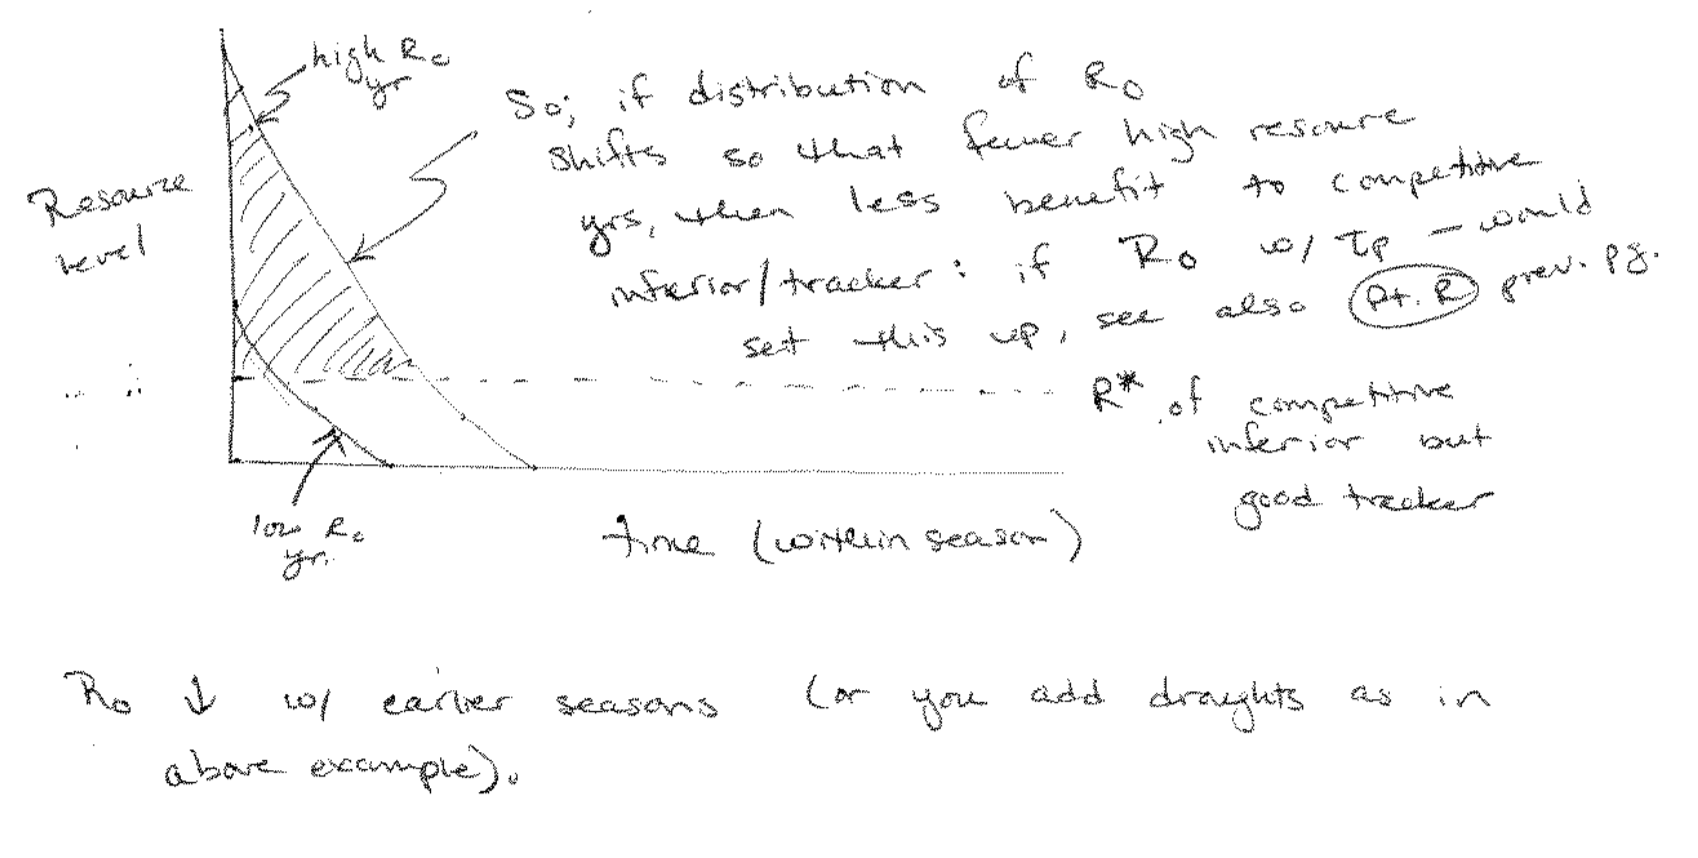
\includegraphics[width=0.9\textwidth]{figure_tradeoff.png}
\caption{{\bf How drought could negatively impact phenological trackers}: Two curves for the same species---a competitively-inferior phenological tracking species---one showing how it responds to a drought (low resource pulse, $R_0$) and another to how it responds in a high drought year (high resource pulse).}
\end{figure}

\newpage
\section{Equations and related notes: January-February 2015}

\noindent Megan's notes from 27 January 2015, following \citet{chesson2003} and \citet{godoy2014}. Note that $j$ is the species index (focal species), $i$ is the invader and $l$ is the supplementary index (that is, all the other species):

\begin{align}
\label{fulleqn} 
N_{j}(t+1) = & (1-d_{j})N_{j}(t) + R_{j}(t)N_{j}(t)  
\\
\label{eqngF} 
g_{j}F_{j} & = \frac{\lambda_{j}}{1+\sum\limits_{l}\alpha_{jl}g_{l,t}N_{l,t}} 
\end{align}

\noindent Breaking down equation \ref{fulleqn} and following how \cite{godoy2014} treats $d$ we can separate $E$ and $C$ in the following way:
\begin{align}
(1-d_{j}) & = \text{ survival in seedbank } = s_{j}(1-g_{j})
\\
R_{j}(t) & = \text{ germination \& death in seedbank } = 0(1-g_{j})(1-s_{j})+g_{j}F_{j} = g_{j}F_{j}
\\
g_{j}F_{j} & = \frac{g_{j}\lambda_{j}}{1+\sum\limits_{l}\alpha_{jl}g_{l,t}N_{l,t}}
\\
& = \underbrace{\ln(g_{j}\lambda_{j})}_\text{$E_{j}(t)$} -\underbrace{\ln(1+\sum\limits_{l}\alpha_{jl}g_{l,t}N_{l,t})}_\text{$-C_{j}(t)$}
\end{align}

\noindent However, this definition of $E$ and $C$ results in $d$ that varies with time because $d$ includes $g{j}(t)$.  How do we avoid this?

\noindent  Currently:

\begin{align}
N_{j}(t+1) = & (1-d_{j})N_{j}(t) + R_{j}(t)N_{j}(t) \\
= & \underbrace{s_{j}}_\text{surv.}\underbrace{(1-g_{j}(t))}_\text{did not germ.}N_{j}(t)+g_{j}(t)F_{j}(t)N_{j}(t)\\
= & s_{j}N_{j}(t) +g_{j}(t)F_{j}(t)N_{j}(t)
\end{align} 

\noindent Alternatively, we can rearrange the equation so that $sN$ is a distinct term (i.e., $d$ does not vary with time).  If we continue to assume a pre-season count, then rearrange:

\begin{align*}
NgF + N(1-g)s*1 + N(1-g)(1-s)*0
\\
gFN + s(1-g)N
\\
sN - sgN + gFN
\\
sN+g(F-s)H
\\
\end{align*}

\noindent Reorganizing the survival and germination terms in this way gives equation:
\begin{align}
N_{j}(t+1) = & (1-d_{j})N_{j}(t) + R_{j}(t)N_{j}(t) \\
= & s_{j}N_{j,t} +g_{j,t}(F_{j,t}-s_{j})N_{j,t}\\
\ln R_{j,t}= & \ln(g_{j,t}(\frac{\lambda_{j}}{1+\sum\limits_{l}\alpha_{jl}g_{l,t}N_{l,t}} -s_{j}))\\
= & \underbrace{\ln g_{j,t}}_\text{$E_{j,t}$} + \underbrace{ \ln(\frac{\lambda_{j}}{1+\sum\limits_{l}\alpha_{jl}g_{l,t}N_{l,t}}-s_{j})}_\text{$-C_{j,t}$}
\end{align}

\noindent  Now that we have defined the general form of the equation, we can calculate the long-term low density growth rate for each species as invader (i.e., invasibility criterion for coexistence).  The long-term low-density growth rate (including temporal but not spatial variability) has three components (Table 1 in \citet{chesson2003}: \textbf{mean fitness}, \textbf{storage effect}, and \textbf{relative nonlinearity}.  

%\noindent  Long-term low-density growth rate: \\
%\begin{align}
%\bar{r_{i}} \approx \underbrace{\bar{r_{i}\prime}}_\text{eq. measures of coexist.} \\
% +& \overbrace{\Delta N_{i}}^\text{rel. nonlin.}\\
% +& \overbrace{\Delta I_{i}}^\text{storage effect})\\
%\end{align}

\noindent  Evaluate the growth rate of each species as invader.  Note that $i$ is for invader, $j$ is any species, and $l$ is a counter to go through all species, with or without invader.

\noindent \textbf{Mean Fitness}
\begin{align*}
\frac{\bar{r_{i}\prime}}{d_{i}} = & \delta \mu_{i} + \delta V_{i}\\
\delta \mu_{i} = & \mu_{i}-\bar{\mu_{l}}^{({l}\neq {i})} \\
= & \mu_{i}-\frac{1}{n-1}\sum\limits_{{l}\neq{i}}^{n}\mu_{l}\\
\mu _{j} = & \langle E_{j} \rangle -\ln d_{j}\\
= &\langle {E_{j}} \rangle -\ln (1-{s_j})\\
\sigma_{j}^{2} = & var(E_{j})\\
\delta V_{i} = & \frac{1}{2}(1-d_{i})\sigma_{i}^{2}-\bar{\frac{1}{2}(1-d_{j}) \sigma_{j}^{2}}^{(j \neq i)}\\
= & \frac{1}{2}(s_{i}\sigma_{i}^{2} - \frac{1}{2}\sum\limits_{l \neq i}^{n}s_{l}var(E_{l})
\end{align*}

\begin{align}
 \langle E_{j} \rangle = & \langle \ln g_{j,t} \rangle \\
\mu_{j} = & \langle \ln g_{j,t} \rangle - \ln(1-s_{j}) \\
\end{align}
\begin{align}
var(E_{j}) = & var(\ln(g_{j,t}))\\
\delta V_{i} = & \frac{1}{2} s_{i} var(\ln(g_{i,t}))-\bar{\frac{1}{2} s_{j} var(\ln(g_{j,t}))}^{(j \neq i)} \\
var(\ln g_{j,t}) = h^2 var(\tau_{p,t}^{2} - 2 \tau_{p,t}\tau_{i})\\
\end{align}
\begin{align}
g_{j,t} = & G_{max} e^{-h(\tau_{p,t}-\tau_{i})^2}\\
\ln g_{j,t} = & \ln G_{max}-h(\tau_{p,t}-\tau_{i})^2\\
\langle \ln g_{j,t} \rangle = & \ln G_{max} - h \langle (\tau_{p,t}-\tau_{i})^2 \rangle\\
& \text{...skipping some intervening equation work...}\\
= & \ln G_{max} - h (\sigma^{2}_{\tau_{p,t}}+(\mu_{\tau_{p,t}}-\tau_{i})^{2})
\end{align}

\begin{align*}
\text{For the case where } \tau_{p} \sim & \beta(p,q)\\
\text{we can calculate the expected value and variance of }&\tau_{p,t} \text{ explicitly}: \\
var (\tau_{p}) = & E \langle \tau_{p}^{2}\rangle - \langle E \langle \tau_{p} \rangle\rangle ^{2}\\
 & var(\tau_{p})+ E \langle \tau_{p}\rangle ^{2} \text{ Megan, is this extra from above or ...?}\\
E \langle \tau_{p} \rangle = & \frac{p}{p+q}\\
var(\tau_{p}) = & \frac{pq}{(p+q)^{2}(p+q+1)}
\end{align*}


\noindent \textbf{Storage Effect}
\begin{align*}
\frac{\Delta I_{i}}{d_{i}} = & \overline{(1-d_{j})\chi_{j}^{(-i)}}^{(j\neq i)} - (1-d_{i})\chi_{i}^{(-i)}\\
= & \sum\limits{j \neq i}^{n} s_j \chi_{j}^{(-i)} - s_{i} \chi_{i}^{-i}\\
\chi_{j}^{(-i)} = & cov(E_{j},C^{(-i)}) \text{ where $C_{(-i)}$ is competition when sp $i$ is invader}\\
\chi_{j}^{(-i)}  = & cov(\ln g_{j,t}, \ln(\frac{\lambda_{j}}{1+\sum \limits_{l \neq i} \alpha_{jl}g_{l,t}N_{l,t}}-s_{j}))\\
\chi_{i}^{(-i)}  = & cov(\ln g_{i,t}, \ln(\frac{\lambda_{i}}{1+\sum \limits_{l \neq i} \alpha_{il}g_{l,t}N_{l,t}}-s_{i}))\\
\end{align*}

\noindent \textbf{Relative Nonlinearity}
\begin{align*}
\frac{\Delta N_{i}}{d_{i}} = & \frac{1}{2}var(C^{(-i)})(d_{i}-\bar{d_{j}}^{(j \neq i)})\\
var(C^{(-i)}) = & var(\ln \frac{\lambda_{j}}{1+\sum \limits_{l} \alpha_{il}g_{l,t}N_{l,t}}-s_{j})\\
\bar{d_{s}}^{(s \neq i)} = & \frac{1}{n-1}\sum \limits_{l=i}(1-s_{l})
\end{align*}

\noindent \textbf{Calculation of ${C_{t}}$}
In Chesson 2003, the calculations in Table 1 are for $C_{t}^{(-i)}$, i.e., the community competition with the invader absent.  In principle this makes sense: if we consider competition experienced by the invader to reflect the level of resource remaining after consumption by all resident species, then  $C_{t}^{(-i)}$ depends only on the identity of the invader.  
For calculate the storage effect, we must calculate the covariance between environment and competion:  $Cov(C_{j,t},E_{j,t}$.  In this case, we can calculate species-specific $C_{j,t}$ and $E_{j,t}$, with $C_{j,t}$ as the annual competition experienced by species $j$, i.e.,
$C_{j,t} = \ln (\frac{\lambda_{j}}{1+\sum\limits{l \neq i}^{n} \alpha_{jl}g_{l,t}N_{l,t}}-s_{j})$
However, when we calculate relative nonlinearity using the equation in Chesson (2003) Table 1, we need to calculate $var(C_{t}^{(-i)})$, which should be the same for all species.  It is not clear how the annual community competitive effect should be calculated.  The denominator in the equation for $C$ is easy to calculate for all but the invader.  But this is multiplied by a species-specific term ($\lambda_{j}$) and a species-specific term is subtracted $s_{j}$.  Therefore, I wonder if the simple equations in Table 1 are not appropriate for this case.  Even if the competitive effects were proportional by species (not the case because of the subtraction of $s_{j}$) then the terms in Table 1 would need to be scaled by $\lambda_{j}$.  \\



\begin{align*}
N_{j} &  \text{ density of adults of species } j \text{ at time } t 
\\
d_{j} & \text{ fraction of adults dying during one unit of time}
\\
R_{j} & \text{ per capita number of new recruits to species} j \text{in the time interval } t \text{ to} + 1
\\
\lambda_{i} & \text{ per-germinant fecundity in the absence of competition}
\\
g_{j} & = 
\\
\alpha_{ij} & = \text{ per capita effect of species } j \text{ on species } i
\\
a_{l} & = \text{ competitive effect of a $sp_{l}$ individual (related to eqn 6 of \cite{chesson2003})
\\ 
\end{align*}

\newpage
\section{Equations and related notes: $R^*$ model}

\noindent For a species \(i\) let (note: see dimensional analysis for full list of current terms, I need to update this here someday):
\begin{align*}
N_{i} & \text{   seedbank of species } i
\\
s_{i} & \text{   survival of seedbank of species } i \text{, buffered pop'ln
  growth occurs via this constant}
\\
\delta & \text{   total time of growing season}
\\
B_{i} &  \text{   biomass of species } i
\\
R &   \text{   resource}
\\
f_{i}(R) & \text{  resource uptake rate of species } i \text{ of } R
\\
c_{i} & \text{   conversion of uptake to biomass of species } i
\\
m_{i} & \text{   partial mortality of species } i
\\
a_{i} & \text{   uptake increase for species } i \text{ as R increases}
\\
\theta_{i} & \text{   shape of uptake of species } i
\\
u_{i}^{-1} & \text{   max uptake of species } i
\\
g_{max,i} & \text{   max germination of species } i
\\
h_{i} & \text{   max rate of germination decrease of species } i
\text{ following a pulse}
\\
\tau_{p} & \text{   time of pulse }
\\
\tau_{i} & \text{   time of max germination of species } i
\\
\epsilon & \text{   abiotic loss of resource}
\\
\phi_{i} & \text{   conversion of biomass of species } i \text{ to
  seedbank, includes overwintering of seeds (as of December 2013)}
\\
b_{i} & \text{   seedling biomass of species } i
\\
\alpha & \text{   phenological tracking of species  } i
\\
\end{align*}

\newpage 
\subsection{Dimensional analysis}
\noindent \emph{Exciting new product as of August 2012, oh la la!}
\begin{center}
\begin{table}[h!]
\caption{Table of parameter values, their definitions and lightweight version of their dimensions (i.e., not yet deemed `grams' or such).}
\begin{tabular}{ | p{3.0cm} | p{6.0cm} | p{4.0cm} |}
\hline 
Parameter & Definition & Unit \\ \hline 
\end{tabular}
\begin{tabular}{ | p{3.0cm} | p{6.0cm} | p{4.0cm} |}
\(N_{i}\) & seedbank of species \(i\) & seeds \\ \hline
\(s_{i}\) & survival of species \(i\) & unitless \\ \hline
\(\delta\) (peak biomass) & total length of growing season & days\\ \hline
\(B_{i}\) & biomass of species \(i\) & biomass \\ \hline
\(R\) & resource & resource\\ \hline
\(c_{i}\) & conversion of \(R\) uptake to biomass of species \(i\) &  \(\frac{\text{biomass}}{\text{resource}}\) \\ \hline
\(m_{i}\) & maintenance costs of species \(i\) & \(\text{days}^{-1}\) \\ \hline
\(a_{i}\) & uptake increase as \(R\) increases for species \(i\) & \(\text{days}^{-1}\) \\ \hline
\(u_{i}\) & max uptake for species \(i\) & \(\frac{(\text{days})(\text{biomass})}{\text{resource}}\) \\ \hline
\(\phi_{i}\) & converesion of biomass to seedbank for species, includes overwintering of seeds \(i\) & \(\text{biomass}^{-1}\), but conceptually \(\frac{\text{seeds}}{(\text{biomass})(\text{seeds})}\) \\ \hline
\(\epsilon\) & abiotic loss of \(R\) &  \(\text{days}^{-1}\) \\ \hline
\(g_{max,i}\) & max germination of species \(i\) & unitless \\ \hline
\(h_{i}\) &  controls the the rate at which germination declines as \(\tau_{p}\) deviates from optimum for species \(i\)  & \(\text{days}^{-2}\) \\ \hline
\(g_{i}\) & germination fraction & unitless \\ \hline
\(\tau_{p}\) & timing of pulse & days \\ \hline
\(\tau_{i}\) & timing of max germination of species \(i\) & days \\ \hline
\(\alpha_{i}\) & phenological tracking of species \(i\) & unitless \\ \hline
\(\theta_{i}\) & shape of uptake for species \(i\) & unitless\\ \hline
\hline
\(b_{i}\) & seedling biomass of species \(i\) & \(\frac{\text{biomass}}{\text{seeds}}\) \\ \hline
\(f_{i}(R)\) & \(R\) uptake \(f(x)\) for species \(i\) & \(\frac{\text{resource}}{(\text{days})(\text{biomass})}\)\\ \hline
\(d_{i}\) & death rate of species \(i\), used in calculations of lifespan & unitless \\ \hline
\(t\) & between year time (formerly T) & years \\ \hline
\(0\) \rightarrow \(\delta\) & within season time (formerly \(\tau\)) & days \\ \hline
\(b_{0}\) & initial biomass per germinant (seed) & biomass \\ \hline
\(\xi\) & \(\frac{\text{final biomass}}{\text{initial biomass}}\) & unitless \\ \hline
\hline
\end{tabular}
\end{table}
\end{center}
\noindent Note for \(\delta\): \(B(t+0)\) is start of season biomass while \(B(t+\delta)\) is the end of season biomass.\\
\noindent Also note: that \(s\) applies to seeds \emph{in} seedbank, while \(\phi\) thus includes some death for current season seeds (see red/blue diagram from 12 May 2014 whiteboard photos).

\newpage
\subsection{System of equations}
\noindent System of equations, for a community of \(n\) species based
on resource competition:
\begin{align*}
N_{i}(t+1) & = N_{i}(t+\delta)s_{i}
\\
\\
\text{where}
\\
\\
N_{i}(t+\delta) & = N_{i}(t) [\text{germination fraction}][\text{seeds
  produced per germinant}]
\\
\\
\text{so then:}
\\
\\
N_{i}(t+1) & =
s_{i}(N_{i}(t)(1-g_{i}(t))+\phi_{i}B(t+\delta)
\\
\\
\text{where:}\\
\\
\frac{\mathrm{d}R}{\mathrm{d}t} & = - \sum_{i=1}^{n}f_{i}(R)B_{i} -\epsilon R\\
\\
\\
\frac{\mathrm{d}B_{i}}{\mathrm{d}t} &  = [c_{i}f_{i}(R) - m_{i}]B_{i}
\\
\\
\text{and the initial condition is:}\\
\\
B(t+0) & = N_{i}(t)g_{i}(t)b_{0,i}
\\
\\
\text{where:} 
\\
\\
g_{i} & = g_{max,i}e^{-h(\tau_{p}-\tau_{i})^2}
\\
\\
f_{i}(R) & = \frac{a_{i}R^{\theta_{i}}}{1+a_{i}u_{i}R^{\theta_{i}}}
\\
\end{align*}

\noindent Adding phenological tracking to model (October 2013 version): \\
\begin{align*}
& \alpha \in 0 \rightarrow 1
\\
&\hat{\tau_{i}} = \alpha \tau_{p} + (1-\alpha)\tau_{i}\\
\end{align*}
\noindent thus:
\begin{align*}
\text{when } \alpha = 0: & \hat{\tau_{i}}=\tau_{i}
\\
\text{when }  \alpha = 1: & \hat{\tau_{i}}=\tau_{p}
\end{align*}

\noindent Getting this into simulation-landia means:
\begin{align*}
B_{i}(0) & = [\text{number of seeds}][\text{germination
  fraction}][\text{seedling biomass}]
\\
\\
\text{which also looks like:}
\\
\\
B_{i}(0) & = N_{i}(t) g_{i}b_{i}
\\
\\
B_{i}(t+\mathrm{d}t) & =B_{i}(t)+[c_{i}f_{i}R(t)-m_{i}]B_{i}(t)\mathrm{d}t
\end{align*}

\subsection{Notes related to equations}

\noindent Also note that I (Lizzie) made one change from the February 2011 board: I think we
used \(h\) accidentally twice for different meanings: one was in the
equation for \(g_{i}\) which we stole from \cite{Chesson:2004eo}
(appendix, see next note), and then one was for the total length of time for the
growing season. Thus I changed this `season-length' \(h\) to
\(\delta\).\\

\noindent Finally, equations for \(\frac{dB_{i}}{dt}, f_{i}(R), g_{i},
\frac{dR}{dt}\) were taken from the appendix of \cite{Chesson:2004eo} (\emph{Oecologia}).\\

\noindent R* does not change with nonstationarity because it is based solely on species-specific characteristics not related to the environment (says Megan, December 2013).

\subsection{Definitions of coexistence}\label{definecoexist}
\noindent In December 2013, we discussed how we will define coexistence. There are a couple options, the second one is better:
\begin{enumerate}
\item Persistence of species in simulations: This is not ideal since you would have to run things a long time and still not know what would truly coexist. But if we do have to do this it is not all bad: if we run stationary then nonstationary environments (one after another, not separate) we can think of it as `here are the species co-occurring. Sure, some may be on Hubbellian random walk to extinction, but that is probably how the real world works anyway.' 
\item Recovery from low-density: For this we need to calculate long-term low density growth rate from either (1) simulations or (2) equations. Equations would be better and would allow us to run stationary and nonstationary simulations separately. This equation should come out of final storage effect equations.
\end{enumerate}


\subsection{How biomass is converted to seed and growing seasons end}


\noindent \emph{The way the growing season ends in the equations is
interesting.} First, as brilliantly stated: the growing seasons ends
[in these equations] when plants stop growing. And, related, the
equations do not deal with setting the end of the growing season. In
my head (Lizzie), abiotic forces can stop a growing season, but in
reality with plant phenology data, the start and end of the growing
season are fundamentally different: at the start species are most
sensitive to abiotic cues and climate change effects are large and
often consistent. For the end of the season climate change effects have been more
muted and variable---suggesting plants in some way do seem to set the
end of the growing season more than abiotic cues do, at least when
compared to the start of season. (And the model follows this.)\\

\noindent \emph{So what we do about it...} It used to happen for all species at $\delta$---so, early species may have peaked and have lower-than-their-peak biomass at $\delta$ while later season species may be at peak. Instead now we let resources go to  the lowest R* and then we take peak biomass (for each species) instead of biomass at $\delta$ (when the growth rate goes below 0), to convert to seeds.


\subsection{Conceptualization of our germination equations}
\noindent A long debate with much thought in October 2013 (see also notes on meeting with Sally Otto, which offers an equation with a clearer cost, but also effectively assumes plants are dumber. Or to say that last bit more positively, `Peter's model assumes plants are smarter,' says Megan). Below are mainly Lizzie's thoughts in December 2013. \\

I think you can compare our formulation to the basically 2-cue system discussed in \citet{Chesson:2004eo}. From pg. 238 he describes how each species basically has a temperature-dependent germination and how far from the pulse is from that optimum determines how much a species germinates each year. Importantly, he notes `The phenological difference in germination discussed
above involves timing that is independent of water
availability, in the sense that rain at the wrong time of
the year or wrong temperature would not bring on
germination or physiological activity.' I can think of two examples you could conceptualize that are similar to this and relevant to the systems we have been thinking about.
\begin{itemize}
\item Snow meltout date in alpine communities as the pulse and temperature requirements (the sum of chilling and spring warming) as the other cue (this maybe works also for some other meadow communities).
\item Nutrient flush date (due to microbial biomass turnover) in temperate systems as the pulse and temperature requirements (again, winter chilling and spring warming together) as the other cues. 
\end{itemize}
These are a little sloppy in that the pulse is supposed to be separate from the cue I think (according to \citet{Chesson:2004eo}, see page 244); but this is sloppy in almost all systems in reality because climate is correlated and evolution means that species probably use that to their benefit.\\

\noindent So, basically I am happy with either the \citet{Chesson:2004eo} formulation or the Otto formulation (which is Table 6.1, model 2 in \cite{chesson2008}, ours is actually also in Table 6.1; it's model 3 but with variable adult biomass). The \citet{Chesson:2004eo} seems one step ahead of Otto: costs in Otto's model would eventually remove most species with \(\tau_{i}\) before the pulse while Chesson says species never germinate before the pulse, they just germinate to varying amounts depending on \(\tau_{p}\).  One benefit of Sally's model though is that it may be better for climate change scenarios because it allows species to make `bad decisions' (if you will) and get hammered for them; as many species have in recent years \citep[e.g.,][]{Inouye:2008gj}.\\

\noindent Note: \(h\) yields different bet hedging strategies.

\subsection{A few assumptions spelled out}
\noindent We assume that:
\begin{enumerate}
\item All species `go' each year, at least a little; that is, we're
  not looking at communities where some species have true
  supra-annual strategies.
\item There is one dominant pulse of the limiting resource (e.g.,
  light or water) at the
  start of each growing season; thus we model a  single pulse per
  season.
\end{enumerate}

\subsection{Simplifying within-year dynamics thoughts}
Can we simplify within-year dynamics to focus on a better model for timing (see photo of October 2013 whiteboard that Megan has)? To rephrase this: Our internal equation is basically R* rankings, so could we create a `deterministic look up table' for the within-year dynamics so we can think more carefully about the timing part of this.  (Related note from 2012 meeting: Decide if we need to ODE solve the intra-annual
  dynamics, then use the discretized version only inter-annually. Note from Lizzie: best ODE solver is now in package `desolve.')

\section{Coexistence with climate change: Notes related to implementing and writing}\label{genoutline}

\subsection{Current outline for paper}
\begin{enumerate}
\item Introduction
\begin{enumerate}
\item Direct and indirect effects of climate change
\item Links to ecological coexistence theory
\item Abiotic shifts expected with climate change: single versus
  synergistic climate shifts
\item Things that will shift with climate change, related to
  coexistence models
\begin{enumerate}
\item Magnitude of and interannual variance in resource pulse (\(R_{\theta}\))
\item Timing of resource pulse (\(\tau_{p}\))
\item Abiotic loss rate of resource (\(\epsilon\))
\end{enumerate}
\item Species traits and climate change: phenological tracking
\item Goals of paper
\end{enumerate}
\item Model description 
\begin{enumerate}
\item Basic storage effect model
\item Our version of the storage effect model
\item Systems for which model is applicable: This is effectively a system with a single large pulse of
resource, that, in a plant-free scenario, is lost exponentially each
year. 
\begin{enumerate}
\item Alpine systems (resource is water): initial large pulse of precipitation from
  snowpack that gradually is used up  throughout season
\item Arid systems? (resource is water): Major pulse of rains (okay, spread out some,
  but really they often concentrate for a couple months and then
  season continues for 3-4 more months)
\item Temperate systems (resource is nutrients): Work with me here, I
  think this is cool. Early in the season turnover of microbes leads
  to a huge flush of nutrients \citep{Zak:1990ar} that microbes (and plants) draw down
  all season. There's no other pulse really---am I crazy here or
  doesn't this work well? (And so microbes draw it down in the
  plant-free case which could easily be affected by climate change,
  e.g., increased temperatures lead to increased microbial activity
  and more rapid draw-down.)
\end{enumerate}
\item Systems it probably doesn't work for: Light-limited systems
  (there is not a single, plant-free decreasing pulse of resource),
  Great Plains or others with multiple pulses.
\item Phenological tracking and the storage effect
\item Our implementation of tracking
\item Derivation of aspects of the storage effect and relative
  non-linearity in our model (this is a big \emph{to do}).
\end{enumerate}
\item Results: Response variables are (1) number of species coexisting, (2) relative shifts in coexistence via storage effect, relative nonlinearity and other factors and (3) the traits of species that persist? Additionally, response variables (probably \(\alpha, \tau_{i}, c_{i}\)) related to how much of a trade-off is needed to offset shifts in coexistence favouring early or tracking species with non-stationary climate change?
\begin{enumerate}
\item Section 1: Shifting abiotic variables
\item Section 2: Species traits: Phenological tracking and shifting
  abiotic variables
\end{enumerate}
\item Discussion
\end{enumerate}

\subsection{Variables of interest}
We consider 3 primary traits of the environment (\(\epsilon, R, \tau_{p}\), which
code to evaporative stress, inter-annual variability, and start of season pulse for our approach basically) and 1
species response trait (phenology, specifically flexibility in
phenology as modeled by a species' ability to shift \(\tau_{i}\)) to model
the dominant expectations of current and future climate change:
\begin{enumerate}
\item \emph{Changes to R:} Shifts in climate means and variability (greater var \(\approx\)
  extreme events) as modeled by changes to \(\mu\) and \(var\) of
    R,
  which can lead to:
\begin{enumerate}
\item Changes in inter-annual covar(E, C)
\item For variability: changes related to buffered population growth:
  for example, when the periodicity of certain extreme events declines
  such that species with certain buffering times no longer get their
  `good' years enough (e.g., periodicity of rainy years every 5 years,
  switches to 10 and the species seedbank is 7 years). This means for
  simulations changing \(var(R)\) must be consider in concert with the
  scale of \(s_{i\cdots n}\).
\end{enumerate}
\item \emph{Changes to \(\epsilon\):} Shifts in climate means that lead to greater abiotic stress on
  environments, as modeled by changes to  \(\epsilon\). For example,
  warmer growing seasons may produce greater evapotranspiration,
  shifting competition for the remaining resource. (By the way, we
  have notes about treating \(\epsilon\) as a function itself.) This should
  affect:
\begin{enumerate}
\item Changes in inter-annual covar(E, C)
\item Note that one basic prediction could be a decline in the storage effect with declines in \(\epsilon\). From \citet{Chesson:2004eo}:
\begin{quote}
... large evaporational [sic] water
losses decrease the contribution of shallow-rooted plants
to soil moisture depletion ... therefore decreasing the link
between uptake and resource shortage .... As
a result, the effectiveness of temporal resource partitioning
by the storage effect would be lower in shallow-rooted
species, because covariance between environment and competition would be less pronounced. Conversely, the
storage effect should be stronger for plants rooted in soil
layers where plant use of water is the dominant mode of
depletion ....
\end{quote}
\end{enumerate}
\item \emph{Changes to \(\tau\):} Longer growing seasons, with several scenarios:
\begin{enumerate}
\item Season is longer (earlier \(\tau_{p}\) but community of species
  do not shift their timing (e.g., no change to  \(\tau_{i \cdots
    n}\)) 
\item Season is longer (earlier \(\tau_{p}\) and some species (`climate-trackers') change
  their timing (community shift in temporal---phenological---synchrony),
  that is (e.g., certain species change to  \(\tau_{i \cdots
    n}\)) such that the distance \(\tau_{p}-\tau_{i}\) is constant
  across years.
\item Could also look at complementarity (histogram of variation in \(\tau_{i \cdots
    n}\); could pull \(\tau_{i \cdots
    n}\) from a beta distribution. (Note: I also wonder if we
  shouldn't just use variation due to above to look at this, versus a
  whole new approach.)
\end{enumerate}
\item How do these variables shift with climate change and co-vary?
\begin{enumerate} 
\item \(R_{\theta}\) increasing inter-annual variance with some giant
  years (extreme events), for snowpack systems it's decreasing
  generally
\item \(\tau_{p}\) getting earlier, also for snowpack systems earlier
  years probably also have higher evaporative stress (\(\epsilon\),
  due to warmer year)
\end{enumerate}
\end{enumerate}


\subsection{How the world changes with climate change}

\noindent In July 2011, I looked at whether the start of spring
has gotten more variable (using some key datasets from NECTAR) and it
hasn't, at all. No change.\\

\noindent \emph{Environmental shifts with climate change, from October 2013 meeting:}\\
Systems we're thinking about (see above) but, effectively, alpine where snowpack meltout is start of season (SOS), nutrient turnover SOS and some precip controlled systems with just one pulse. 
\begin{enumerate}
\item \(\tau_{p}\) will get earlier in many systems (alpine and nutrient), not sure on precip---there it might just get more variable
\item \(\epsilon\) increase in mean and increase in extreme events (this seems pretty possible across a lot of systems---good one)
\item \(R_{0}\) increase or decrease in mean maybe (who knows what happens in precip system), increase in variance (for precip systems), increase in extreme events 
\item Correlations in \(\tau_{p}\) and \(\epsilon\) - this basically says `does the first day of the growing season correlate with the average temperature of the growing season?' which, yeah, is weird. Lizzie thinks there's probably a weak positive covariance here (just because there's a lot of noise in annual weather but wet soils hold cold, and dry soils hold heat so \emph{all other things being equal} you could see this correlation. From an email from Ben Cook from 30 May 2013:
\begin{quote}
So, both Europe and the Northeast US have had super crappy springs in March and April (so annoying!). Mostly it was due to an almost unprecedented negative swing of the NAO, which just funneled lots of cold arctic air in the region. As for the summer? Harder to tell. If an area gets lots of rain in the spring, it can mean really wet soil which can keep things cooler in the summer. But other than that, we don't really have much skill in predicting summer time climate. 
\end{quote}
Otherwise, not sure anyone has looked at this at all in precip systems and for snowpack there may be something here since Pederson et al. 2011 says that snowpack control has basically shifted from precipitation control to temperature control so with climate change you could start seeing a correlation in alpine systems between \(\tau_{p}\) and \(\epsilon\) (which is kind of cool, but sort of something that is not low-hanging, obvious fruit -- or maybe it's low hanging fruit and only obvious to us).
\item Correlations in \(\epsilon\) and \(R_{0}\) maybe for alpine you could see, with climate change, increases in \(R_{0}\)  and decreases in \(\epsilon\), but we're still bickering on this and what \(\epsilon\) really is (incident irradiance vs. relative humidity?)
\item Correlations in \(R_{0}\) and \(\tau\) nothing to date or in future? Maybe in alpine systems?
\end{enumerate}

So, where did we arrive at after all this? Even though we used to be interested in correlated shifts in these we're not so much anymore. Instead the \emph{best place to start} seems to be: earlier \(\tau_{p}\) and increases in \(\epsilon\) and \(\epsilon\) extreme events. Then maybe move on to \(R_{0}\) (mean and extreme events). And again, just skip correlations.\\

Note that increased extreme events for \(\epsilon\)  will effectively reduce biomass (you could also consider modeling this so it ties to \(m_{i}\) or modify \(g_{i}\) to lead to total loss, perhaps).\\

While here, though, I will mention that we discussed \emph{which} correlations will shift with climate change and the big one seems to be the North American alpine story: where the relationship between how \(\tau_{p}\) affects mortality has shifted with species' \(\tau_{i}\) such that there is now higher mortality imposed on species with earlier \(\tau_{i}\). We did briefly discuss how to model this and think maybe the best way is to add in, external to the within-year integral, a fraction that germinated and died as a f(x) of \(\tau_{i}\)  and frost event time.\\

\subsection{Species differences: How to thoughts}
\noindent New notes as of October-December 2013: \emph{Models without tracking:}\\
How will we adjust the equations for simulations about shifts in the environment? For now we plan to let parameters vary some and see if we can pick out patterns. If this gets tricky we can switch to trade-offs between \(\tau_{i}\) and \(c_{i}\). \\

Note that one possible trade-off is earlier \(\tau_{i}\) could correlate with lower competitive ability, which is mentioned in \citet{Chesson:2004eo} on page 245: Coexistence would be promoted
only when this temporal pattern entails tradeoffs, e.g.,
when later pulse users are able to draw down soil moisture
to lower levels than are early users.\\

(Old question from October 2013, maybe should cut): Do we need to make sure that for all \(i\), \(\int g_{i}\) are equal, or is it that \(\int g_{i}(t)\tau_{p}(t)\mathrm{d}t\) should be constant (the latter being the average of \(g_{i}\) weighted by the distribution of \(\tau_{p}\) through time).\\

\noindent \emph{Models with tracking:}\\
In nature early species have quicker-return investments on growth and early is often high tracking, so it's hard to tell whether early \emph{or} high-tracking trades off with this quicker-return angle. So what we plan on doing:\\
\noindent For now, for coexistence: we'll trade off \(c_{i}\) and \(\tau_{i}\), when we add in alpha we'll leave this above trade-off and maybe:
\begin{itemize}
\item get some coexisting species and add high tracking randomly to all and see what happens
\item get some coexisting species and add high tracking to the early ones and see what happens
\item add weak versus strong tracking
\end{itemize}

\noindent \emph{Comparisons with competition/colonization trade-offs:} Can think of trade-off as competition-colonization one: rapid response to resource availability (colonization) versus special case of competition.\\

Without tracking we may predict benefits to early-colonizers decline with earlier seasons. As start-date moves earlier, early folks lose benefit (assuming they tend to often go at optimum time) and you get more late folks. Late species may be less different than one another---and less responsive to environment. Early folks, effectively, become more similar to environment. 

\newpage
\section{Tracking thoughts \& fun}\label{trackingthoughs}
In August 2012 Megan came up with a new way to model phenological tracking, it's linear and better than the one presented here. We also discussed three key ways to think of tracking:
\begin{enumerate}
\item Species can have fixed flowering/leafing (not track).
\item Species can phenologically track pulse.
\item Species can phenologically track something at least at one time in history correlated with the pulse.
\end{enumerate}
We agreed that while (3) is interesting---would allow you to look at mismatch ideas etc.---(1) and (2) have more biological support for plants and are interesting enough in and of themselves, so we will focus on and model (1) and (2) and not (3).\\

\noindent In August 2013 an issue we worried about: Will tracker always win? Answers: No, not if it's a poor competitor, that is, if it responds quickly to resource pulse but then does poorly at low resource levels. I also think it's important to remember that not all tracking species will track perfectly so some species should grow before trackers some years, when their fixed \(\tau_{i}\) corresponds well to \(\tau_{p}\). Also, we have a note that high intraspecific competition could dampen trackers, especially when greater than interspecific competition.\\

\noindent New things we came up with that we want to look at in regards to {\bf phenological tracking}. First off, we have a lot of versions of similar questions. 
\begin{itemize}
\item Has climate change made tracking more advantageous? Or, how prevalent is tracking in a stationary versus nonstationary system? Basically, one hoped-for outcome (by Lizzie) is to show that with stationary climate tracking strategies and non-tracking strategies may coexist happily, but when you add nonstationarity the world shifts that tracking is so strongly favoured as to make non-tracking rare or to require a very huge trade-off etc.. So we have a bunch of related questions to this:
\begin{itemize}
\item How big do trade-offs have to be for tracking to be non-advantageous (to allow coexistence with other species)?
\item Another angle, is tracking the dominant strategy with a shifting environment (distribution) vs. stationary environment distribution?
\end{itemize}
\item Follow up from October 2013: How much does climate have to shift (non-stationarity in system) given some level of fitness differences trading off with tracking for tracking to become the dominant strategy?
\end{itemize}
{\bf It would be great to add real data here!} Some options: First, Lizzie may be able to track down information about negative correlations between tracking and competitive abilities (for nutrient resources). This would put some of the trade-off questions in perspective. Next, we could also see  \emph{what we know about climate projections} and from there see how big do the trade-offs have to be with climate change to make non-tracking a feasible strategy strategy (this `feasible' and `dominant' terminology is a little wobbly; I admit that)?\\

\noindent This tracking angle matches to the `Generalists, specialists and plasticity' section of \citet{Chesson:2004eo}. You could imagine by removing the benefit of trade-offs associated with not being plastic, then nonstationarity could favour generalists (plastic species, that is). Here's the most relevant bit (according to Lizzie):
\begin{quote}
However, plasticity, or any generalist resource consumption
behaviors, including those involving drought resistance,
may come at a cost .... In such circumstances, there is no
contradiction that a generalist can coexist with specialists
so long as the specialists are in fact superior performers
during the times or conditions that favor them, and there 
are some times when no specialists are favored so that the
generalist is then superior.
\end{quote}

As of August 2015 we decided {\bf against doing tracking with joint distributions} (see notes above\ref{phenCCpaper}), but here are the old notes on it:
\begin{quote}
Next up, I need to work on how to make joint distributions in R (all different types, not just multivariate normal ones) so we can link \(\alpha_{i}\) with \(c_{i}\). For this I need to look into copulas and the R package \verb@copula@. See also these pages:\\
\url{http://www.r-bloggers.com/copulas-made-easy/}\\
\url{https://sites.google.com/a/wisc.edu/jed-frees/multivariate-regression-using-copulas}
\end{quote}


\newpage
\section{Notes on megadroughts paper}\label{mayannotes}
\begin{center}
{\Large Temporal redness, Mayan megadroughts and Californian invaders\\ or\\ Red noise and the sunset of Mayans and European invaders}
\end{center}

\noindent Can we use this model to test if certain strategies (say, high tracking) can increase over shorter timescales but be completely excluded from this system given rarer, long-term (red) periods of environmental `harshness'?\\

To expand: My theory works as such: If a closed population of a species has a relatively short length for its buffered population growth---for example, imagine an annual grass with a 3 year seedbank---and enters a new system where the climate has long term fluctuations, could that population possibly do well during certain environmental phases, but be completely excluded (local extinction) during others. For example, the scenario of California annual invasive grasses: they do great now, but less well in drought years and large very long droughts (Mayan megadroughts are part of the ENSO cycle, possibly, and are decade or multi-decadal) could possibly throw them entirely out of the system. Thus the answer to the question I always get: If European annual grasses do so well in coastal sage scrub why weren't there any native annual grasses? would be---wait a while and  then you'll see. \\

There is also an evolutionary angle to this: short lifespans and short seedbanks with these sorts of long-term cycles could lead to evolving quickly, during one climate phase, towards a damn stupid strategy when the next climate phase kicks in. But I don't want to go there, just to point it out.\\

\noindent Opportunity to coin new term (from one term I hate and one that I like): {\bf invasion extinction debt}, the number of invaders that would go extinct if you wait a very long time. \\

\noindent We could bring Ben Cook on this project to give us some info on how frequencies of droughts have shifted over the past 2K years or so in North America. Or, maybe we could look at some shifts in drought periodicities globally just to press home the message that these can vary a lot across time. 

\section{Storage effect notes}

\subsection{Miscellaneous notes}

\noindet The lost paper: \emph{Shifting drivers of coexistence with climate change}, which includes all the work to date (December 2013), plus phenological tracking.\\

\noindent {\bf Predictions:} Even though we are not shifting \(var(R_{0}), var(\tau_{p}), var(\epsilon)\) we are shifting E (species' responses to environment) and thus \(var(E)\) may increase. That could be cool.\\

\subsection{Notes on coexistence mechanisms}
We spent a substantial amount of time carefully working through Chesson 1994.  A few notes on how this might apply to nonstationarity
\begin{itemize}
\item In the General Model, growth rate is divided into E and C components.  To examinte the effects of fluctuations using a Taylor approximation, r is examined around E*, C*, where growth rate is 0.  
\item  The model is reparameterized in terms of curly-E, curly-C, which is the complete growth function, reparameterized around C* and E*, respectively.  To make the taylor approximation, it is limimted to variability around E*, C* of order O2
\item the approximation is also limited to the behavior of the function around the point E*,C*, such that if the curvature of the function changed at a point far from E*, C*, this nonlinearity would not be captured.
\item  the approximations are made with the assumption of a stationary process, without temporal autocorrelation and drawn from the same distribution through time.  This approximation is the one that makes studying nonstationarity with these approximations difficult. 
\item  we came up with a couple ideas about how coexistence mechanism partitioning might still be useful, even without stationarity.  For example, you could compare coexistence and coexistence mechanisms present at the beginning and end of a period of change.  The likely outcome is that species will continue to persist after they shoudl have gone extinct because of lags.  It is hard to think of a case when the converse would be true, at least under the case of mean change.  If the variance is changiing, then the outcomes are less obvious and might include increased coexistence
\end{itemize}
I worked through Section 4: Analysis of the General Model, however, actually doing those calculations with any particular model is tricky, particularly making an assumption for E*,C*.  Using Section 5.5 as an example, I tried to work through the calculations for our simple model.  Equation 95 is largely equivalent to our simple model. The only difference is that we originally parameterized competition as $(1+ \sum\limits_{j=1}^{j=n}g_{j,t}*X_{j,t}*\alpha_{ij})$, but equation 96 has competition as a simple sum, with no additional +1. %Lizzie changed the above a little to make math work, may want to check  

Section 5.5 is the same as our simplified model.  Understanding through Equation 99 is clear.  Table II lists the parameters of the seedbank model, and the definition of these terms is clear.  To understand the terms in Table III, we still need to define rho and sigma and to make the correct assumption about the value of E* and C*.  The assumptions around E*, C* are a sticking point and where I got stuck. 
Looking back at the notes now, however, it seems like there may still be some room forward here.  We are proceeding on the simulations, but Megan will spend a little more time to see if we can actually make the calculations in Table III.

\subsection{Tiny notes about the storage effect to help Lizzie}
\noindent The 3 ingredients of the storage effect are:
\begin{enumerate}
\item differential response to the environment (subadditivity)
\item covar(E, C)
\item buffered population growth
\end{enumerate}

\noindent Ingredients for the storage effect \emph{in our model:}
\begin{itemize}
\item buffered population growth: \(s_{i}\)
\item variable response to the environment: \(\tau_{i}\), which generates:
\item \(covar(E,C)\)
\end{itemize}

\section{Miscellaneous notes}
\noindent We keep an eye on who has cited Chesson et al. 2004
and for actual modeling work it's just Chesson, and for that it's all
his seed predation work.\\

\noindent More random notes: \citet{Chesson:2000vd} (pg. 354) \(r\) holds temporal variation in \(\delta I\) and \(\delta N\) so effectively:\\
- species can coexist via intra-annual temporal mechanisms (for example, maybe this is what most mid-season species in the mesic temperate zone do), and/or\\
- species can coexist via inter-annual temporal mechanisms (maybe early-season species in most mesic temperate environments)\\

\subsection{Some notes for writing}
\begin{enumerate}
\item Understanding the variable responses of communities and species
  due to climate shifts is a major aim of current
ecology.
\begin{enumerate}
\item Varied responses
\begin{enumerate}
\item reversed phenology \citep{yu2010} 
\item downhill shifts \citep{Crimmins:2011dq}
\end{enumerate}
\item Effects of climate change extend well beyond shifts in the mean
\end{enumerate}
\item Models of community assembly in ecology build upon coexistence
  via environmental variability.
\item Launch into set-up.
\end{enumerate}
\noindent Some key refs we worked with:
\citep{Chesson:1993gi,Chesson:2000ak,Chesson:2000vd,Chesson:2004eo}. Some
papers using storage effect model or Armstong and McGhee with field
data: \citep{Angert:2009,Kuang:2008ri,Kuang:2009rj,Levine:2009ym}.\\

\subsection{Some random notes from the whiteboard}
\noindent Relative nonlinearity is:
\begin{align*}
\left(\frac{d^{2}}{dR^{2}}\right)(var(R))
\end{align*}
\noindent Non-additivity (\(\gamma\)) is (in general, still working on
what it is for our equations) when considering population growth
(\(r_{i}\)):
\begin{align*}
r_{i} & = \omega_{i}(E_{i}, C)
\\
\\
\gamma & = \frac{\partial \omega}{\partial E \partial C} 
\end{align*}

\noindent but, what is \(E\) and \(C\) in our system?
\begin{align*}
C & = - \sum_{i=1}^{n}f_{i}(R)B_{i} \rightarrow f_{i}R
\end{align*}
\noindent is this (above) the response to
  competition? An alternative note we had with many question marks
  was:
\begin{align*}
covar(E,C) \approx covar\left(R_{i}, \sum_{i=1}^{n}B_{i}\right)
\end{align*}

\subsection{Small, somewhat random, but \emph{fascinating} questions} 
\noindent So what does it mean if species co-exist in the same community via mechanisms operating on totally different timescales?\\

\noindent  New random query: Is there humidity without plants?\\

\noindent  Also, someday, you could wonder if earlier \(\tau_{p}\) allows for more niche space for species at the end of the season that have a really low R*.\\

\noindent  \emph{Also, totally random note for Lizzie:} Trees use previous year' resources to flush leaves/flowers in current year.



\newpage
\section{References}
\bibliography{/Users/Lizzie/Documents/git/bibtex/LizzieMainMinimal}
\bibliographystyle{/Users/Lizzie/Documents/git/bibtex/styles/ecolett.bst}

\newpage
\section{Almighty figure aspirations} 
\noindent Figure 3 and 4 are ideas from Lizzie as of 11 December 2013, see also some older figure ideas at end of the paper (from 2011). 

\begin{figure}[h!]
\centering
\noindent 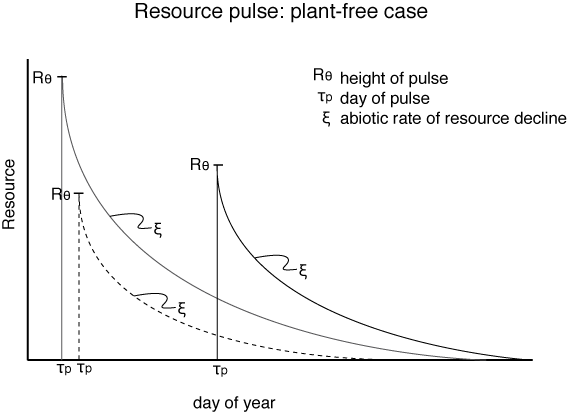
\includegraphics[width=0.8\textwidth]{varenv_varying.png}
\caption{{\bf Major coexistence variables directly affected by
    climate change}  We focus on three major coexistence variables
  that have been (or will be) influenced by climate change---a couple
  examples of how varying them changes the resource pulse (without plants).}
\end{figure}

\newpage
\begin{figure}[h!]
\centering
\noindent 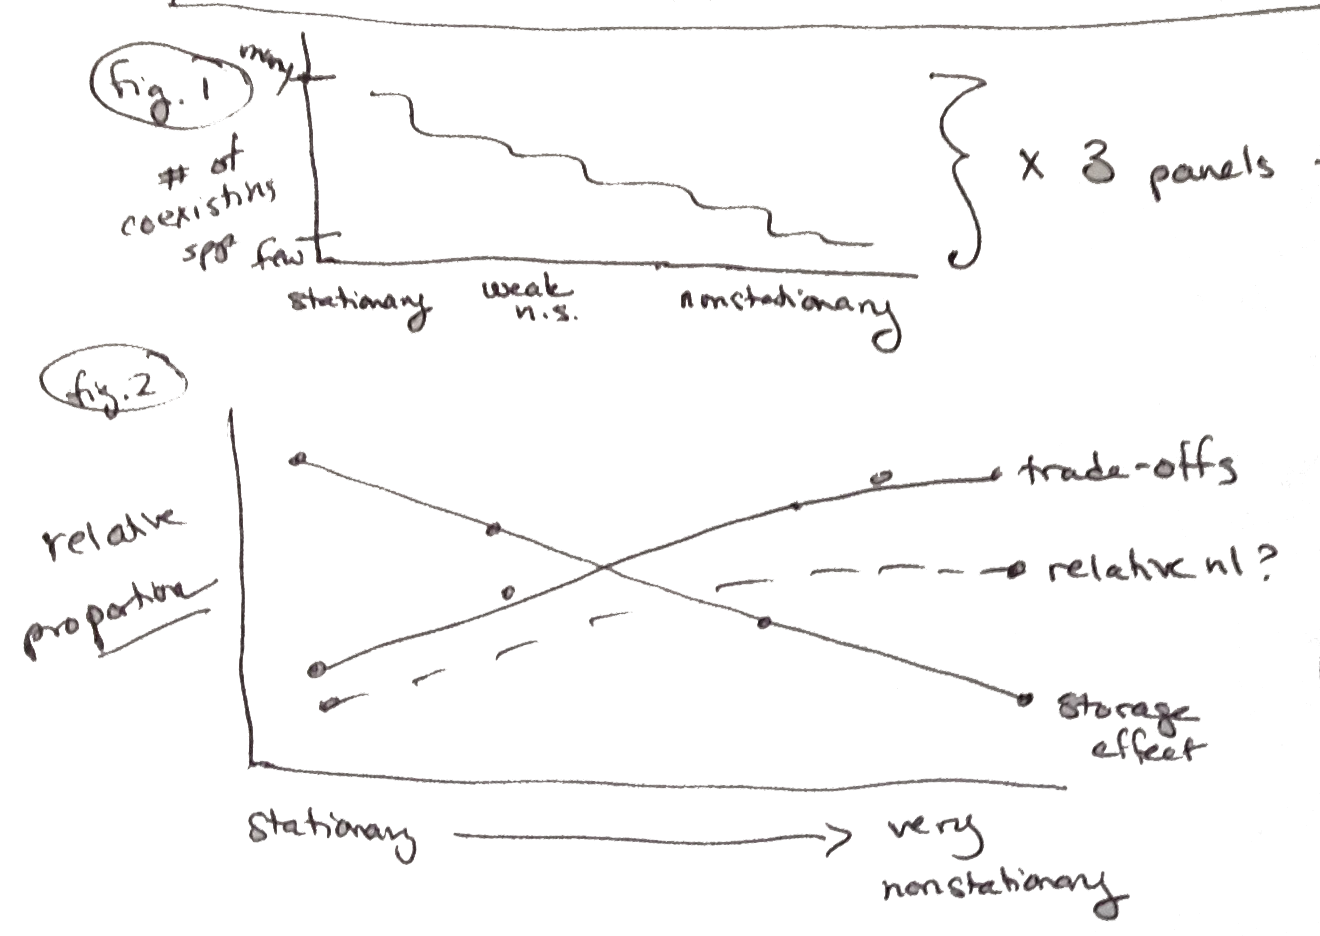
\includegraphics[width=0.8\textwidth]{figurehopes_MoC.png}
\caption{{\bf How does climate change affect mechanisms of coexistence?} Two figures: the first is simple it's just the number (or percent of total possible) of species coexisting; the second figure is to look at how mechanisms shift with scenarios that are stationary, weakly nonstationary or strongly nonstationary. Each of these figures should be one panel for each variable manipulated (\(\epsilon, \tau_{p}\) and maybe \(R_{0}\)).}
\end{figure}

\newpage
\begin{figure}[h!]
\centering
\noindent 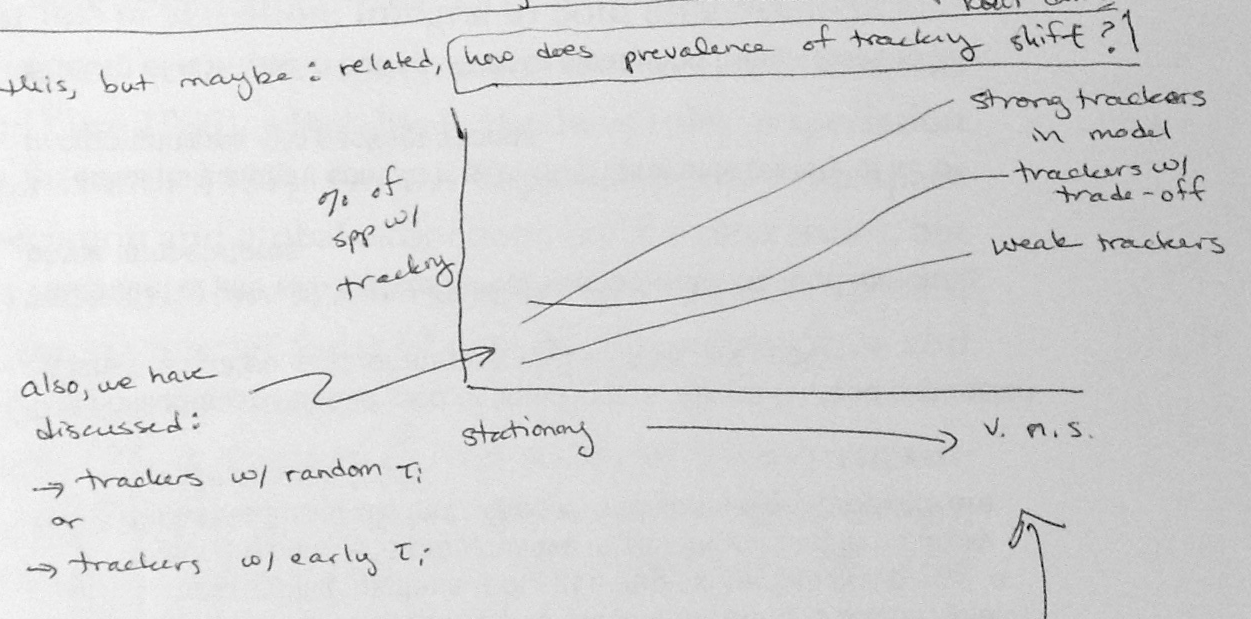
\includegraphics[width=0.8\textwidth]{figurehopes_tracking.png}
\caption{{\bf How does the prevalence of tracking shift with nonstationarity?} See the section on tracking questions above for the full plethora of questions related to this (e.g., this is also the realm of how strong does the negative correlation between tracking and competitive ability have to be to make tracking non-advantageous). But, basically we want to look at how tracking shifts in stationary versus nonstationary systems. So we could do something like this (we also discussed looking at trackers with random \(\tau_{i}\) versus trackers with early \(\tau_{i}\) as you usually see in nature) and/or we could re-do the mechanisms of coexistence figures above with trackers in the mix.}
\end{figure}


\end{document}

